\documentclass{report}
\usepackage[parfill]{parskip} % Replaces \setlength{\parindent}{0pt}
\usepackage{hyperref} % For clickable links and bookmarks
\usepackage{bookmark}

\usepackage{booktabs}
\usepackage[utf8]{inputenc}
\usepackage{enumitem}
\usepackage{amsmath} % For math environments
\usepackage{tcolorbox}
\usepackage{array}
\usepackage{xcolor}
\usepackage{algorithm}
\usepackage{algorithmic}
\definecolor{chaptergreen}{HTML}{1B8110}

\makeatletter
\def\chapter{\@ifstar\@schapter\@chapter}
\def\@chapter#1{%
  \refstepcounter{chapter}%
  \addcontentsline{toc}{chapter}{\protect\numberline{\thechapter}#1}%
  \chaptermark{#1}%
  {\par\vspace{2em}\centering\LARGE\bfseries
   \textcolor{chaptergreen}{Chapter \thechapter\\#1}\par\vspace{1em}}%
}
\def\@schapter#1{%
  {\par\vspace{1em}\centering\LARGE\bfseries
   \textcolor{chaptergreen}{#1}\par\vspace{1em}}%
}
\makeatother

% ------------------------------
% Packages
% ------------------------------
\usepackage{graphicx}      % For including images
\usepackage{amsmath}       % Advanced math typesetting
\usepackage{amssymb}       % Math symbols (e.g., \mathbb, \leqslant, etc.)
\usepackage{amsthm}        % Theorem/lemma environments
\usepackage{stmaryrd}      % Extra math symbols (e.g., semantic brackets ⟦ ⟧)
\usepackage[short]{datetime} % Date formatting
\usepackage{caption}       % Custom captions for figures/tables
\usepackage{subcaption}    % Subfigures (side-by-side images)
\usepackage{multicol}      % Multi-column layout (e.g., notes, problems)
\setlength{\columnseprule}{1pt} % Vertical line between columns
\usepackage{soul}          % Highlighting (\hl{})
\sethlcolor{yellow}        % Highlight color
\usepackage[margin=1.75cm]{geometry} % Page margins

% ------------------------------
% Theorem Environments
% ------------------------------
\theoremstyle{definition} % Non-italic style for definitions/remarks
\newtheorem{remark}{Remark}
\newtheorem{theorem}{Theorem}
\newtheorem{lemma}{Lemma}
\newtheorem{definition}{Definition}
\newtheorem{corollary}{Corollary}
\newtheorem{property}[theorem]{Property}      % Shares counter with theorem
\newtheorem{proposition}[theorem]{Proposition} % Shares counter with theorem

% ------------------------------
% Custom Math Commands
% ------------------------------
% Vectors (boldface)
\newcommand{\xx}{\mathbf{x}}
\newcommand{\yy}{\mathbf{y}}
\newcommand{\uu}{\mathbf{u}}
\newcommand{\rr}{\mathbf{r}}
\newcommand{\vv}{\mathbf{v}}
\newcommand{\ww}{\mathbf{w}}
\newcommand{\aaa}{\mathbf{a}}
\newcommand{\bb}{\mathbf{b}}
\newcommand{\cc}{\mathbf{c}}
\newcommand{\ee}{\mathbf{e}}
\newcommand{\0}{\mathbf{0}}
\newcommand{\ii}{\mathbf{i}}
\newcommand{\jj}{\mathbf{j}}
\newcommand{\kk}{\mathbf{k}}


% Transformations / Matrices
\newcommand{\Tx}{T(\xx)}
\newcommand{\Ai}{A^{-1}}   % Inverse
\newcommand{\At}{A^{T}}    % Transpose

% Spaces
\newcommand{\Rn}{\mathbb{R}^n}
\newcommand{\Rm}{\mathbb{R}^m}
\newcommand{\Pn}{\mathbb{P}_n} % Polynomials of degree ≤ n
\newcommand{\mxn}{m \times n}  % Matrix dimensions

% Subspaces
\newcommand{\Col}{\mathrm{Col}\;}  % Column space
\newcommand{\Row}{\mathrm{Row}\;}  % Row space
\newcommand{\Nul}{\mathrm{Nul}\;}  % Null space
\newcommand{\Span}{\mathrm{Span}\;} % Span
\newcommand{\rank}{\mathrm{rank}\;} % Rank

% Bases / Coordinate systems
\newcommand{\BB}{\mathcal{B}}  % Basis B
\newcommand{\CC}{\mathcal{C}}  % Basis C
\newcommand{\cB}{[\xx]_\BB}    % Coordinates of x in basis B
\newcommand{\cC}{[\xx]_\CC}    % Coordinates of x in basis C
\newcommand{\xB}[1]{[#1]_\BB}  % Custom coord notation (input)
\newcommand{\xC}[1]{[#1]_\CC}  % Custom coord notation (input)
\newcommand{\pb}{P_\BB}        % Projection onto basis B
\newcommand{\pbc}{P_{\CC \leftarrow \BB}} % Change of basis B → C
\newcommand{\pcb}{P_{\BB \leftarrow \CC}} % Change of basis C → B

\newcommand{\samplevec}{\aaa = \langle a_1, a_2, a_3 \rangle}

\newcommand{\parx}{\frac{\partial z}{\partial x}}
\newcommand{\pary}{\frac{\partial z}{\partial y}}


% Matrix shortcuts
\newcommand{\matAI}{$\begin{bmatrix}A & I\end{bmatrix}$} % Augmented matrix [A|I]


\newcommand{\vect}[2]{\begin{pmatrix} #1 \\ #2 \end{pmatrix}}

\title{15-382 Collective Intelligence}
\date{First Edition}
\author{Salman Hajizada}

\begin{document}
\maketitle

\chapter*{Disclaimer}
This document aims to summarize the content of the slides for 15-382, including
what the author considers important. As always, the definition of important is
highly subjective so the author might have omitted something that was
important to another person, or included something that is trivial to another.


Good luck,

SH

\chapter*{Dynamical Systems}

\section*{Fingerprints of Complex Systems}

\begin{itemize}
    \item Multi-agent / multi-component
    \item Decentralized
    \item Local interactions
    \item Dynamic
\end{itemize}

\section*{Types of Abstract Models:}

\begin{description}
    \item[Agent-based] Mechanistic implementation of the multi-component interactions.
    \item[Mathematical (white-box)] Formally describe the relations among the relevant components.
    \item[Black-box] Input-output pairs from the system are used to predict...
    \item[Statistical] Describing patterns and correlations between variables.
\end{description}

\section*{Systems of ODEs}

Here is a system of $n \ge 1$ Ordinary Differential Equations
\[
\begin{cases}
\frac{dx_1}{dt} = f_1(\xx(t))\\
\frac{dx_2}{dt} = f_2(\xx(t))\\
\vdots \\
\frac{dx_n}{dt} = f_n(\xx(t))
\end{cases}
\]
where $\xx(t)$ is an $n$-dim vector.


A continuous-time Dynamical System is defined by a system of differential equations:
\[
\frac{d\xx(t)}{dt} = \mathbf{f}(\xx, t; \theta) \quad \text{or} \quad \dot{\xx} = \mathbf{f}(\xx, t; \theta)
\]
where $\mathbf{f}: \Rn \to \Rn$ specifies how each component of the state evolves as $t$ changes.
It can depend on a set of given parameters $\theta$

\textbf{Some definitions:}

\begin{itemize}
    \item Initial conditions: where the system is at the beginning of the evolution:
    $\xx(t_0)$
    \item Phase space: space of all possible states
    \item Trajectory: the curve traces by $\xx(t)$ in the phase space starting from $\xx(t_0)$
    \item Solution: is in the form $\xx(t; t_0)$ that defines a family of time trajectories
    in the phase space. Once we fix $t_0$, we fix a unique trajectory
\end{itemize}

\section*{Vector fields and flows}
How are solutions built? At any point, $\mathbf{f}$ assigns a vector
that shows where the point is heading (direction of motion).

If we plot these arrows (vectors) in the phase space, we get can
get an idea of how the system evolves.

\textbf{Flow: } $\Phi: \mathtt{R} \times \Rn \to \Rn$ is the collection of
all trajectories generated by all possible starting conditions.

$\Phi(t, \xx_0) = \xx(t; \xx_0)$


A fundamental theorem guarantees
that \textbf{two orbits corresponding to two different initial solutions never intersect with
each other }, except at equilibrium

\section*{Basic Properties}

An ODE is linear if
\begin{itemize}
    \item $\mathbf{f}(\xx) = A\xx$ (Homogeneous)
    \item $\mathbf{f}(\xx) = A\xx + b$ (Affine)
\end{itemize}

Linear ODE enjoys closed form solutions, non-linear ODEs usually not


A system is autonomous if time doesn't appear in expression of $\mathbf{f}$.

Facts:
\begin{itemize}
    \item Any $n$-order ODE can be rewritten as a system of $1$st order ODEs in $\Rn$
    \item Any Non-Autonomous ODE can be rewritten as an autonomous one
\end{itemize}

So we will focus on 1st order, autonomous and linear ODEs

\section*{Solving!}
\begin{center}
    
\includegraphics[width=0.2\textwidth]{images/cat.png}
\end{center}

General form of linear ODE:
\[
\dot\xx = A \xx, \quad x \in \Rn
\]

A solution is a function $\xx(t)$ that satisfies the vector field $A$.

(Lots of derivation out is skipped, here's how to solve)

\begin{enumerate}
    \item Solve $\det(A - \lambda I) = 0$ for $\lambda$
    \item The roots $\lambda_i$ are eigenvalues of $A$
    \item For each $\lambda_i$, there exists a non-null eigenvector
    $\uu_i$
    \item Together they yield one solution: $\xx(t) = \uu_i e^{\lambda_i t}$
    \item Each distinct eigen-pair gives ONE independent vector solution
    \item The general solution is then the combination of these terms:
    $\xx(t) = c_1 e^{\lambda_1 t} \uu_1 + \dots + c_n e^{\lambda_n t} \uu_n$ (at most n terms)
\end{enumerate}

Important: the above is strictly true only if all eigenvalues are distinct

Matrix Exponential representation: $\xx(t) = e^{A t} \xx(0)$ where $\xx(0)$ is a generic initial condition

\section*{Exponentials and Asymtotic Behavior}

Since the solution is a sum of exponentials, stuff is being pulled in the direction of the eigenvectors,
weighted by their corresponding signed eigenvalues.


If the real part of $\lambda_i > 0$, mode $i$ is unstable/diverging.

If the real part of $\lambda_i < 0$, mode $i$ is stable/contracting.

At each point, the solution \textbf{mixes} the modes.

\section*{Equilibrium points}

A state $\xx_e$ is an equilibrium state of a system $\dot\xx = \mathbf{f}(\xx)$ if
when at a time $t_0$ the sytem is at $\xx_e$ then it stays there FOREVER

Why? Velocity of the field in $\xx_e$ is null: $\mathbf{f}(\xx_e) = 0$


For a linear ODE, the equilibrium points are the points of the \textbf{Null Space} (solutions to $A \xx = 0$)
Theres one trivial solution at $\xx = \0$ if $A$ is invertible, o.w. inifnitely many solutions

\section*{Taxonomy of equilibria}

\begin{table}[h!]
\centering
\renewcommand{\arraystretch}{1.3}
\setlength{\tabcolsep}{8pt}
\begin{tabular}{>{\bfseries}m{3.5cm} m{6cm} m{5cm}}
\textbf{Equilibrium Type} & \textbf{System’s Behavior} & \textbf{Trajectories} \\
\midrule
Equilibrium state &
If at or arrives at $\mathbf{x_e}$, it stays at $\mathbf{x_e}$ &
Trajectory is constant: $\mathbf{x}(t) = \mathbf{x_e}$ \\

Stable equilibrium (Lyapunov) &
If started close to $\mathbf{x_e}$, stays close to $\mathbf{x_e}$ forever &
Nearby trajectories remain in a neighborhood of $\mathbf{x_e}$ \\

Asymptotically stable equilibrium &
If started close to $\mathbf{x_e}$, stays close to $\mathbf{x_e}$ and moves toward $\mathbf{x_e}$ as $t \to \infty$ &
Nearby trajectories converge to $\mathbf{x_e}$ \\

Unstable equilibrium &
Even if started very close to $\mathbf{x_e}$, eventually diverges from $\mathbf{x_e}$ &
Nearby trajectories diverge from $\mathbf{x_e}$ \\
\bottomrule
\end{tabular}
\end{table}

\begin{center}
    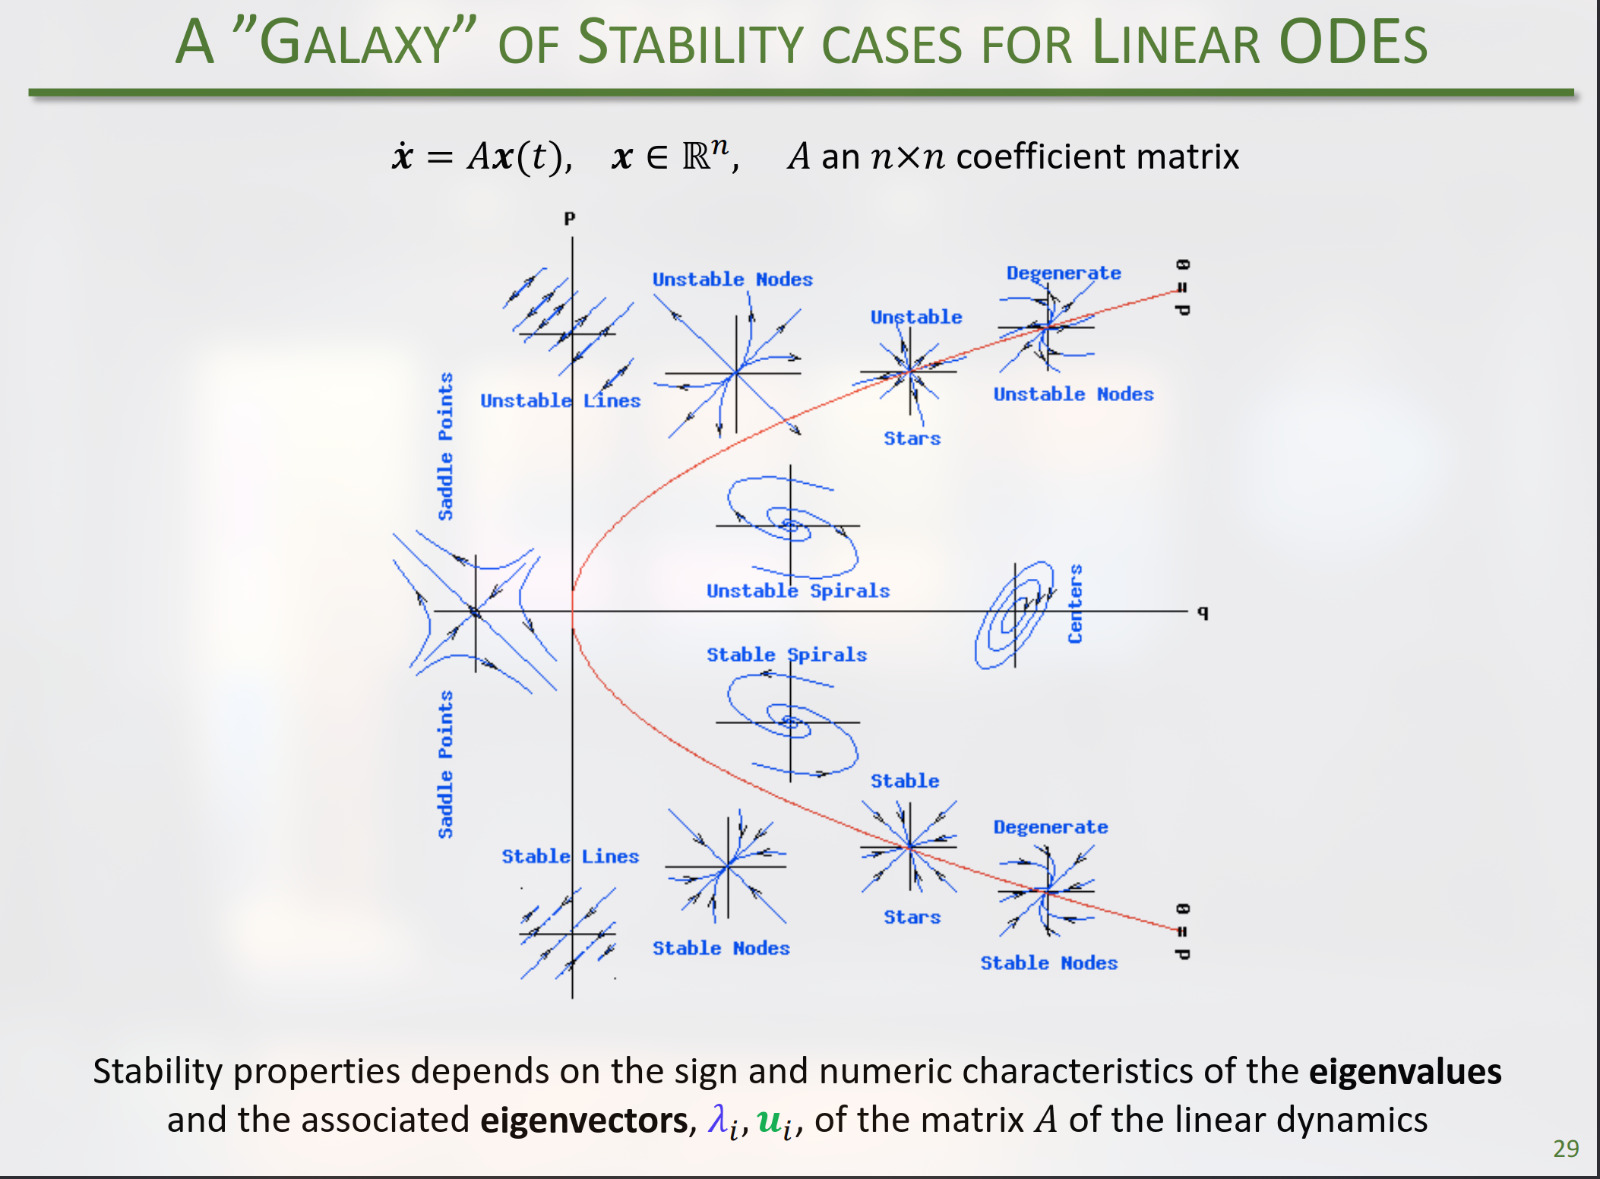
\includegraphics[width=0.6\textwidth]{images/image.png}
\end{center}

\section*{Linear System Classification by Eigenvalues}

% Consider the linear system:
% \[
% \dot{\mathbf{x}} = A\mathbf{x}, \quad A \in \mathbb{R}^{2\times 2}
% \]
% We classify equilibria based on the eigenvalues of \( A \).


% \textbf{1. Two Distinct Real Eigenvalues of Opposite Sign}

% Behavior:
% \begin{itemize}
%   \item Trajectories diverge along one eigenvector and converge along the other.
%   \item Equilibrium is a \textbf{saddle point (unstable)}.
% \end{itemize}

% \textbf{2. Two Distinct Real Eigenvalues with Same Sign}

% Behavior:
% \begin{itemize}
%   \item \textbf{Stable node} if both eigenvalues $< 0$.
%   \item \textbf{Unstable node} if both eigenvalues $> 0$.
%   \item Trajectories are straight lines along eigenvectors.
% \end{itemize}

% \textbf{3. One Repeated Real Eigenvalue, Two Independent Eigenvectors (Star / Proper Node)}

% Behavior:
% \begin{itemize}
%   \item Repeated real eigenvalue (algebraic multiplicity = 2).
%   \item Two linearly independent eigenvectors.
%   \item Trajectories are straight lines toward/away from the origin.
%   \item \textbf{Stable} if $\lambda < 0$, \textbf{unstable} if $\lambda > 0$.
% \end{itemize}

% \textbf{4. One Repeated Real Eigenvalue, One Eigenvector (Improper / Degenerate Node)}

% Behavior:
% \begin{itemize}
%   \item Repeated real eigenvalue with only one eigenvector.
%   \item Requires a generalized eigenvector.
%   \item Trajectories are curved, tangent to the direction of the eigenvector.
%   \item \textbf{Stable} if $\lambda < 0$, \textbf{unstable} if $\lambda > 0$.
% \end{itemize}

% \textbf{5. Complex Eigenvalues with Nonzero Real Part (Spiral / Focus)}

% \[
% A =
% \begin{pmatrix}
% a & -b\\
% b & a
% \end{pmatrix}, \quad
% \lambda_{1,2} = a \pm bi
% \]

% \[
% \mathbf{x}(t) = e^{at}
% \begin{pmatrix}
% \cos(bt) & -\sin(bt)\\
% \sin(bt) & \cos(bt)
% \end{pmatrix}
% \mathbf{x}(0)
% \]

% \textbf{Behavior:}
% \begin{itemize}
%   \item Complex conjugate eigenvalues.
%   \item \textbf{Stable spiral} if $a < 0$, \textbf{unstable spiral} if $a > 0$.
%   \item Trajectories rotate while exponentially approaching or diverging from origin.
% \end{itemize}

% \textbf{6. Pure Imaginary Eigenvalues (Center)}

% \[
% A =
% \begin{pmatrix}
% 0 & -\omega\\
% \omega & 0
% \end{pmatrix}, \quad
% \lambda_{1,2} = \pm i\omega
% \]

% \[
% \mathbf{x}(t) =
% \begin{pmatrix}
% \cos(\omega t) & -\sin(\omega t)\\
% \sin(\omega t) & \cos(\omega t)
% \end{pmatrix}
% \mathbf{x}(0)
% \]

% \textbf{Behavior:}
% \begin{itemize}
%   \item Purely imaginary eigenvalues, no real part.
%   \item Trajectories are closed orbits (circles or ellipses).
%   \item Neither converge nor diverge — \textbf{neutrally stable}.
% \end{itemize}

(for the saddle case, keep in mind a product is negative only
if exaclty one of the numbers is negative)

\renewcommand{\arraystretch}{1.1} % less vertical space
\begin{tabular}{|c|c|c|}
\hline
\textbf{Eigenvalues} & \textbf{Critical Point} & \textbf{Stability} \\
\hline
$r_1, r_2 > 0$ & Node (real, distinct) & Unstable \\
$r_1, r_2 < 0$ & Node (real, distinct) & Asymptotically stable \\
$r_1 r_2 < 0$ & Saddle & Unstable \\
$r_1 = r_2 \neq 0$ & Node / Improper node & Same as sign of $r_1$ \\
$r_{1,2} = \lambda \pm i\mu$ & Spiral (focus) & Same as sign of $\lambda$ \\
$r_{1,2} = \pm i\mu$ & Center & Neutrally stable \\
\hline
\end{tabular}

\section*{Perturbations}

For Pure Imaginary Eigenvalue,
small perturbations add a tiny real part to the eigenvalues:

\begin{itemize}
    \item $\lambda > 0$ (positive real part) $\implies$ trajectories spiral outward (unstable spiral).
    \item $\lambda < 0$ (negative real part) $\implies$ trajectories spiral inward (stable spiral).
\end{itemize}

For Repeated Real Eigenvalues

\begin{itemize}
    \item If the eigenvectors are linearly independent, the system stays a node, but may change to a saddle if the signs differents.
    \item If the eigenvectors are linearly dependent (a degenerate node),
    a small perturbation will typically turn it into either a spiral
    (if eigenvalues become complex) or a node
    (if eigenvalues become distinct real numbers).
\end{itemize}

\section*{Linearization around a Critical Point}

Consider a nonlinear system:
\[
\dot{\mathbf{x}} = \mathbf{f}(\mathbf{x}), \quad \mathbf{x} \in \mathbb{R}^n
\]

Let $\mathbf{x}_0$ be a critical point: $\mathbf{f}(\mathbf{x}_0) = 0$.

\textbf{Step 1: Linear Approximation}

\[
\mathbf{f}(\mathbf{x}) \approx \mathbf{f}(\mathbf{x}_0) + J_{\mathbf{f}}(\mathbf{x}_0)(\mathbf{x} - \mathbf{x}_0)
\]

Since $\mathbf{f}(\mathbf{x}_0) = 0$, the linearized system is
\[
\dot{\mathbf{x}} \approx J_{\mathbf{f}}(\mathbf{x}_0) (\mathbf{x} - \mathbf{x}_0), \quad
\mathbf{y} = \mathbf{x} - \mathbf{x}_0
\]

\textbf{Step 2: Jacobian Matrix}

\[
J_{\mathbf{f}}(\mathbf{x}_0) =
\begin{bmatrix}
\frac{\partial f_1}{\partial x_1} & \cdots & \frac{\partial f_1}{\partial x_n} \\
\vdots & \ddots & \vdots \\
\frac{\partial f_n}{\partial x_1} & \cdots & \frac{\partial f_n}{\partial x_n}
\end{bmatrix}_{\mathbf{x} = \mathbf{x}_0}
\]

\textbf{Step 3: Eigenvalues, Eigenvectors, and General Solution}

Compute eigenvalues $\lambda_i$ and eigenvectors $\mathbf{v}_i$ of $J_{\mathbf{f}}(\mathbf{x}_0)$.
The general solution of the linearized system is
\[
\mathbf{y}(t) = \sum_{i=1}^n c_i e^{\lambda_i t} \mathbf{v}_i, \quad
\mathbf{x}(t) = \mathbf{x}_0 + \mathbf{y}(t)
\]

\textbf{Step 4: Stability Analysis}

Stability is determined by the eigenvalues of the Jacobian $J_{\mathbf{f}}(\mathbf{x}_0)$, just like in the linear case.

\section*{Global Behavior and Nullclines}

\begin{itemize}
  \item \textbf{Basin of Attraction:} The set of all initial conditions that eventually lead a trajectory to the same stable equilibrium point.
  \item \textbf{Separatrix:} The boundary between different basins of attraction.
  \item \textbf{Isoline:} The set of points where a function takes the same value.
  \item \textbf{Isocline:} The set of points where the vector field has the same \textbf{slope}.
  \item \textbf{Nullcline:} A specific type of isocline. It's the set of points where the slope is either zero or infinite (i.e., where one component of the vector field is zero).
\end{itemize}

Nullcline fun facts:
\begin{enumerate}
  \item The \textbf{$x$-nullcline} is the curve where $\dot{x} = f(x,y) = 0$.
  \item The \textbf{$y$-nullcline} is the curve where $\dot{y} = g(x,y) = 0$.
  \item On the $x$-nullcline, the vector field has no horizontal component, so vectors can only point vertically (up or down).
  \item On the $y$-nullcline, the vector field has no vertical component, so vectors can only point horizontally (left or right).
  \item \textbf{Equilibrium points} are exactly at the intersection of the $x$-nullclines and $y$-nullclines (since $\dot{x}=0$ and $\dot{y}=0$ simultaneously).
  \item Nullclines divide the phase space into regions. In each region, the sign of $\dot{x}$ and $\dot{y}$ is constant.
\end{enumerate}

\section*{Limit cycles}

\textbf{A periodic orbit} is just any trajectory that forms a closed loop.

\textbf{A limit cycle} is an isolated closed trajectory.
This means neighboring trajectories are not closed; they either spiral into the limit cycle (a stable limit cycle) or spiral away from it (an unstable limit cycle).
There's also mixed scenarios (half-stable)

Example: Van der Pol Oscillator

\section*{2D is Boring}

\begin{theorem}
Any closed trajectory muyst encolse at least one equilibrium
\end{theorem}
\begin{theorem}{Poincare-Bendixson Theorem:}

IF a trajectory is trapped in a closed, bounded region R,

AND this region R contains no equilibrium points,

THEN the trajectory must eventually approach a limit cycle.
\end{theorem}

In other words, 2D systems cannot have chaos

\section*{Chaos and Strange Attractors}

3 main types of attractors: Fixed Points, Limit Cycles and Strange Attractors (the last
appears only in 3D+)

Properties of strange attractors:
\begin{itemize}
  \item Sensitive dependence on initial conditions: two initial conditions very
  close to each other become very far apart as time goes on (but remain confined in the set
  that defines the attractor)
  \item Fractal dimensions (e.g. $2.06$). Non-integer
\end{itemize}

\textbf{Example: Lorenz Attractor}
\begin{enumerate}
  \item For a parameter r=21, trajectories spiral into one of two stable fixed points.
  \item For r=28, the fixed points become unstable. Trajectories are still
  bounded, but they never settle down. They move from one "wing" of the
  attractor to the other in an aperiodic, unpredictable way.
\end{enumerate}

\begin{definition}
Chaos: \textbf{aperiodic long-term behavior} in a \textbf{deterministic} system that exhibits
\textbf{sensitive dependence on initial conditions}
\end{definition}

\chapter*{Iterated Maps}

\section*{Intro}

\textbf{Discrete-time dynamical systems} have a state which is only 
defined at integer steps. 

The state is:
\[\xx(n) = (x_1(n), \dots, x_k(n))\] 
where $k$ is the dimension of the system and $n$ is an integer step parameter

and the rule is:

\[\xx(n) = \mathbf(f)((\xx(n-1), \dots, \xx(n-m)))\] (so the system here depends on 
$m$ previous states)

Can also be written nicely as $\xx_n = \mathbf{f}(\xx_{n-1}, \dots, \xx_{n-m})$

Next state is obtained by directly apply the map $\mathbf{f}$

\section*{1D Iterated Maps and Cobweb Plots}

We focus on the simplest case: a 1D map $x_n = f(x_{n-1})$

\begin{itemize}
    \item \textbf{Orbit:} sequence of points generated starting at $x_0$
    and keep applying the map 
    \item \textbf{Fixed point:} Point that maps to itself: $f(x^*) = x^*$
\end{itemize}

\textbf{Sawtooth diagram:} Plotting the $(x, f(x))$ diagram. No time shown, 
all it tells you is if the system is at $x$ now, the next state will be at $f(x)$

\textbf{Cobweb Plot construction algorithm:}

\begin{enumerate}
    \item Draw $y=f(x)$ and $y=x$
    \item Start at initial point $x_0$ on horizontal axis 
    \item Move \textbf{vertically} to $y = f(x)$ (this is point $x_0, x_1$)
    \item Move \textbf{horizontally} to $y = x$ (this is point $x_1, x_1$)
    \item Move \textbf{vertically} to $y = f(x)$ again (this is point $x_1, x_2$)
    \item Keep going lil bro
\end{enumerate}

The intersections of $y = f(x)$ and $y = x$ are fixed points. We can analyze 
stability of a fixed point by looking at the plot.

\section*{Stability of fixed points}

Some simple derivation because its interesting:

Consider a point near a fixed point, $x_n = x^* + \epsilon_n$. 
Next point $x_{n+1} = f(x^* + \epsilon_n) = f(x^*) + f'(x^*)\epsilon_n + O(\epsilon_n^2)$

So a linear approximation shows that $\epsilon_{n+1} = f'(x^*)\epsilon_n$. Let $\lambda = f'(x^*)$

Solving: $\epsilon_n = \lambda^n \epsilon_0$. If you know some basics you can 
infer stability from this alone but I will write a table.

\begin{table}[h!]
\centering
\renewcommand{\arraystretch}{1.2}
\begin{tabular}{lll}
\toprule
\textbf{$\lambda = f'(x^*)$} & \textbf{Stability Type} & \textbf{Behavior Near $x^*$} \\
\midrule
\multicolumn{3}{l}{\textbf{Stable (Attracting)}} \\
\quad $0 < \lambda < 1$ & Monotonic & Converges from one side \\
\quad $-1 < \lambda < 0$ & Oscillatory & Zig-zag convergence (alternating sides) \\
\quad $\lambda = 0$ & Superstable & Very fast convergence \\
\addlinespace
\multicolumn{3}{l}{\textbf{Unstable (Repelling)}} \\
\quad $\lambda > 1$ & Monotonic & Diverges from one side \\
\quad $\lambda < -1$ & Oscillatory & Alternating divergence \\
\addlinespace
\multicolumn{3}{l}{\textbf{Marginal}} \\
\quad $|\lambda| = 1$ & Neutral & Linearization inconclusive \\
\bottomrule
\end{tabular}
\end{table}

\section*{Logistic map and chaos}

\textbf{Logistic Map:} $x_{n+1} = r x_n (1 - x_n)$ where $x_n \in [0, 1]$ is 
population, $r \in [0, 4]$ is growth rate

\begin{itemize}
    \item $1<r<3$: The population converges to a single, stable fixed point $x^*=1-1/r$.
    \item $r=3$: The fixed point becomes unstable.
    \item $3<r<3.449\dots$: The system no longer settles to one point. It settles into a stable period-2 cycle, oscillating between two values. This is a bifurcation.
    \item $r>3.449\dots$: The 2-cycle becomes unstable and splits into a stable period-4 cycle. This continues, creating an 8-cycle, 16-cycle, etc., in a period-doubling cascade.
    \item $r>r^{\inf} \approx 3.5699\dots$: The cascade finishes, and the system enters the chaotic regime. The orbit becomes aperiodic, never settling down and seemingly random.
\end{itemize}

This behavior can be summarized in an orbit diagram .
\begin{itemize}
    \item The x-axis is the parameter r.
    \item The y-axis plots the long-term attractor points for that r.
\end{itemize}    

A \textbf{bifurcation} is a qualitative change in the long-term behavior
of a system with a smooth variation of a parameter
    
A bunch of math deriving Lyapunov Exponents, but here is the final result:

\[\lambda = \lim_{n \to \inf} \frac{1}{n} \sum_{k=0}^{n-1} \ln|f'(x_k)|\]

The approximation for $\lambda$ can be constructed numerically, by iterating the map!
\begin{itemize}
    \item $\lambda < 0$: For stable fixed points and cycles
    \item $\lambda > 0$: For chaotic attractors
    \item $\lambda = 0$: This is the marginal case, which occurs at bifurcation points.
    \item $\lambda$ is the same for all points in the basin of attraction of an attractor
\end{itemize} 
    


\chapter*{Cellular Automata (CA)}

\section*{CA properties}

A \textbf{Cellular Automaton} is a multi-dimensional discrete-time dynamical 
system that is defined by 
the principle of locality. properties: 

\begin{description}
    \item[Systems's state is $n$-dimensional] $\xx(t) = (x_1(t), \dots, x_n(t))$
    \item[Discrete time]: updated at discrete time steps 
    \item[State components arranged according to a given topology] 
    \item[Neighborhood defined based on topology]: $N(x_i) = 
    {x_j : x_j \text{ is a neighbor of }x_i}$

    Neighborhood is the range for a cell to be influenced by other cells

    1D Example: $N(x_i)={x_{i-1},x_i,x_{i+1}}$

    2D Examples:
    \begin{itemize}
        \item Von Neumann: The cell and its 4 neighbors (up, down, left, right).
        \item Moore: The cell and its 8 surrounding neighbors (a 3x3 box).
    \end{itemize}

    \item[Locality of updates]: Each state component $x_i$ evolves according to a rule 
    that depends only on its own state and those of its neighbors in $N(x_i)$.

    Local-state transition function, $F_i: S(N(x_i)) \to S_i$ where $S_i$
    s the set of values that state component $x_i$ can take, 
    and $S$ is the state values from the cells in the neighborhood set.

    \item[Initial Conditions]: state at $t=0$
\end{description}

\section*{Lattices and Boundaries:}
\textbf{Infinite/adaptive lattice}: The grid grows as the pattern propagates

\textbf{Finite lattice}
\begin{itemize}
    \item Hard boundary: fixed, edge cells have a fixed state
    \item Hard boundary: reflective, leftmost (rightmost) cell only diffuse right (left)
    \item Soft boundary: periodic boundary conditions, edges wrap around
\end{itemize}

\section*{Updating Schedules:}
\begin{itemize}
    \item Synchronous Updating: At time t, all cells read the states of 
    their neighbors. Then, they all compute their next state. Finally, all cells update their state simultaneously to begin step $t+1$.
    \item Asynchronous Updating: Cells update one at a time or in random groups. The order matters. A cell updating later in the step will see the already updated states of its neighbors who updated earlier.
\end{itemize}

\section*{Some Math}
We assume they are homogeneous (same lattice, same N, and same rule F for all cells)
and use synchronous updating.

\textbf{Combinatorics}
Let: 
\begin{itemize}
    \item $k = |S|$ is the number of states per cell 
    \item $M$ is the number of cells 
    \item $r$ is the range ($floor(|N(a)|/2)$)
\end{itemize}

Then: 
\begin{itemize}
    \item Number of possible state configs: $k^{M}$
    \item Number of possible neighborhood configurations: $k^{|N|}$
    \item Number of possible evolution functions (rules): $k^{\left(k^{|N|}\right)}$
    Why? This is the number of possible functions mapping from the set of neighborhood configurations (domain size $k^{|N|}$) to the set of possible next states (codomain size $k$). For each of the $k^{|N|}$ possible inputs, there are $k$ possible outputs.
\end{itemize}

\section*{Wolfram Code}

For Wolfram's 1D CA: $S = \{0, 1\}$ (so $k=2$) and the neighborhood is $r=1$ (i.e., $N(x_i) = \{x_{i-1}, x_i, x_{i+1}\}$, so $|N|=3$).

Using our formula, the number of rules = $k^{\left(k^{|N|}\right)} = 2^{\left(2^3\right)} = 2^8 = 256$.


\section*{Four classes of Behavior and Chaos}

\renewcommand{\arraystretch}{1.3}
\begin{table}[h!]
\centering
\begin{tabular}{|c|p{4cm}|p{4cm}|c|}
\hline
\textbf{Class} & \textbf{Behavior} & \textbf{Information Dynamics} & \textbf{Lyapunov Exponent} \\
\hline
1 & Evolves to a simple, stable, homogeneous state (all 0s or all 1s). & Small changes die; information is lost. & $\lambda \le 0$ \\
\hline
2 & Evolves to simple periodic structures (stripes, oscillators). & Small changes may persist locally but do not spread. & $\lambda = 0$ \\
\hline
3 & Evolves to chaotic, aperiodic patterns (e.g., Rule 30). & Small changes spread out and affect distant regions. & $\lambda > 0$ \\
\hline
4 & Creates complex, localized, moving structures. (e.g., Rule 110 is \textbf{Turing complete}) & Small changes may or may not spread; irregular but structured dynamics. & $\lambda > 0$ (tends to 0) \\
\hline
\end{tabular}
\end{table}

\section*{Game of Life}

\begin{itemize}
    \item 2D Lattice of identical cells 
    \item Moore neighborhood
    \item 2 states: dead or alive
    \item The 4 Rules:
    \begin{description}
        \item[Loneliness] A live cell with $<2$ live neighbors dies.
        \item[Overcrowding] A live cell with $>3$ live neighbors dies.
        \item[Survival] A live cell with 2 or 3 live neighbors lives on.
        \item[Reproduction] A dead cell with exactly 3 live neighbors becomes alive.
    \end{description}
    \item Garden of Eden: A pattern that can only exist as initial pattern. In other
words, no parent could possibly produce the pattern.
\end{itemize}

\chapter*{Networks}

\section*{Basic Graph Theory, Terminology, Properties}

\textbf{Graph:} two sets $(V, E)$ of vertices/nodes and 
edges/arcs/links 

Can be directed (interaction flows one way) or undirected (interaction flows both ways)

For Undirected graphs:
\begin{itemize}
    \item Node degree $k_i$: number of edges adjacent to 
    node $i$
    \item Handshake theorem: let $L$ be the number of edges.
    Then $L = \frac{1}{2}\sum_{i=1}^{N}k_i$
    \item Average degree: $\langle k \rangle = \frac{2L}{N}$
\end{itemize}

For Directed Graphs:
\begin{itemize}
    \item In-degree: number of edges going into node 
    \item Out-degree: number of edges going out of the node 
    \item Total degree $k_i = k_i^\text{in} + k_i^\text{out}$
    \item Average degree (either in or out): $\frac{L}{N}$
\end{itemize}

\textbf{Degree Distribution:} $p_k = \frac{N_k}{N}$ where $N_k$ is number of 
nodes with degree $k$

In real networks degree distribution is highly heterogeneous

\textbf{Complete graph:} every possible edge is there. $L = \frac{N(N-1)}{2}$

In real networks, the number of edges is way less than that.


\begin{itemize}
    \item \textbf{Walk:} A sequence of vertices (and corresponding edges) such that consecutive vertices are adjacent. 
    Vertices and edges may repeat. For example, $(1 \to 2 \to 1)$ is a valid walk.

    \item \textbf{Path:} A walk in which all vertices (and therefore all edges) are distinct. 
    For example, $(1 \to 2 \to 3)$ is a path, but $(1 \to 2 \to 1)$ is not.

    \item \textbf{Length:} The number of edges in a walk or path, or the sum of their weights if the graph is weighted.

    \item \textbf{Distance:} The length of the shortest path between two vertices. 
    In unweighted graphs, this equals the minimal number of hops; in weighted graphs, the minimal total weight.

    \item \textbf{Shortest Path:} A path whose length equals the distance between its endpoints.

    \item \textbf{Diameter:} The maximum distance between any two vertices in the graph; equivalently, 
    the length of the longest shortest path.
\end{itemize}

\textbf{Connected graph} is an undirected graph where there exists a path between 
every pair of nodes

For directed graphs there is 
\begin{itemize}
    \item Strongly connected if for every pair there is a path 
    \item Weakly connected if every pair there is a path \textbf{when you
    ignore edge directions}
\end{itemize}

If the largest component in a graph has a large fraction of the nodes,
we call it the giant component

\section*{Two representations for graphs}

\begin{enumerate}
    \item Adjacency list: a mapping from each node to it's neighborhood
    \item Adjacency matrix: $N \times N$ matrix $A$ such that $A_{ij} = 1$ if link 
    $(i, j)$ exists, and $0$ otherwise. 
\end{enumerate}

\textbf{More about adjacency matrices}
\begin{enumerate}
    \item For undirected graphs they are symmetric
    \item Number of walks between nodes $i, j$ can be calculated as follows:
        $(A^l)_{ij}$ gives $\#$walks of length $l$.
\end{enumerate}

\section*{Some measures}

\textbf{Average path length:}
\[
h = \frac{1}{2E_{\text{max}} \sum_{i, j \ne i}h_{ij}}
\]
where $h_ij$ is the distance from $i$ to $j$ and $E_{\text{max}} = n(n-1)/2$

\textbf{Clustering Coefficient}

Let $L_i$  be the number of links between neighbors of $i$. 
Then the clustering coefficient of node $i$ is 
\[
c_i = \frac{2L_i}{k_i(k_i - 1)}
\]

\textbf{Global clustering coefficient:} $C = \frac{1}{N}\sum_{i=1}^{N}c_i$

\section*{Properties of real networks}
Real networks are: 
\begin{itemize}
    \item Scale-free (from $p_k$): they have hubs
    \item Small world (from $h$): average distance is very small 
    \item Locally dense (from $C$): clustering is very high
\end{itemize}

We will try to have a process that can create a network with these properties 

\section*{Model 1: Erdos-Renyi (ER)} I DO NOT CAREEEEE ABOUT THE DOTS ABOVE THEIR NAMES 


\textbf{Generative process:} each of the $\binom{N}{2}$ possible edges, an edge is created with 
probability $p$
\textbf{Degree Distribution:} 
\[
p_k = \binom{N-1}{k}p^k (1-p)^{N-1-k}
\]
Mean degree is $\bar{k} = p(N-1)$, Variance is $(N-1)p(1-p)$

For large, sparse networks that simplifies to Poisson distribution:
\[
p_k = e^{-\bar{k}} \frac{\bar{k}^k}{k!}
\]

\textbf{Clustering Coefficient:} $E[C] = p = \frac{\bar{k}}{N-1}$, i.e. small

\textbf{Average path length} grows as: $O(\log N)$

\textbf{Verdict:}
\begin{enumerate}
    \item Scale-free: NO, $p_k$ is Poisson (should be power law)
    \item Small world: YES, low $h$
    \item Locally dense: NO, $C$ is very low (should be high)
\end{enumerate}

\section*{Model 2: Watts-Strogatz (WS) (Small World)}

This model was made to fix the clustering problem. 

\textbf{Generative process:}
\begin{enumerate}
    \item Start with a regular ring lattice, where each node is connected to 
    $m$ nearest neighbors. Graph starts with high $C$ and $h$
    \item Go through each edge, and with prob $p$ rewire one end of the edge 
    to a randomly chosen node. 
\end{enumerate}

What happens for different p?
\begin{itemize}
    \item $p = 0$: Just a regular lattice, high $C$ and $h$
    \item $p = 1$: Just a random graph, low $C$ and $h$
    \item $p = 0.01$: A few rewired links act as shortcuts, dropping 
    $h$ dramatically (to around $log N$), while keeping a high $C$
\end{itemize}

\textbf{Verdict:}
\begin{enumerate}
    \item Scale-free: NO, $p_k$ is peaked at around $m$
    \item Small world: YES, low $h$
    \item Locally dense: YES, $C$ is high 
\end{enumerate}

We are almost there

\section*{Model 3: Barabasi-Albert (BA) Scale-Free Model}

\textbf{Generative Process}

Two main new mechanisms:

\begin{enumerate}
    \item \textbf{Growth:} The network is not a fixed size. It starts with a small "seed" 
    network, and at each time step, a new node is added.
    \item \textbf{Preferential Attachment:} New node connects to $m$ existing nodes. 
    The probability $\Pi(i)$ of it connecting to an existing node $i$ is not uniform. 
    It is proportional to that node's current degree $k_i$:
    \[
    \Pi(i) = \frac{k_i}{\sum_{j}k_j}
    \]
\end{enumerate}

Rich get richer, rich nodes have higher chance of getting new links

\textbf{Verdict:}
\begin{enumerate}
    \item Scale-free: YES, naturally produces a power-law degree distribution ($p_k$ around $k^{-3}$)
    \item Small world: YES, low $h$
    \item Locally dense: KINDA, $C$ is a typically lower than in real networks
\end{enumerate}

\section*{Summary of Network Models}

\renewcommand{\arraystretch}{1.2}
\setlength{\tabcolsep}{8pt}
\begin{tabular}{|l|c|c|c|}
\hline
\textbf{Model} & \textbf{Scale-Free?} & \textbf{Small World?} & \textbf{High Clustering?} \\
\hline
Erdos-Renyi (ER) & No & Yes & No \\
Watts-Strogatz (WS) & No & Yes & Yes \\
Barabasi-Albert (BA) & Yes & Yes & Kinda \\
\hline
\end{tabular}

\section*{Importance of a node: Network Centrality Measures}

Certain positions within the network give nodes more power or importance.
We will explore different types

\section*{Classic (Non-Recursive) Centrality Measures}

\textbf{Degree Centrality}

The number of other nodes $n$ is connected to. 

\textbf{Meaning:} A node with high degree centrality 
has high potential communication activity

\textbf{Betweenness Centrality}

Number of shortest paths connecting all pairs of other nodes that pass through $n$

\textbf{Meaning:} A node with high betweenness centrality acts as a "bridge" or "gatekeeper"
and has significant control over the flow of information.

\textbf{Closeness Centrality}

Measures how "close" a node is to all other nodes in the network.

\[
C(n) = \frac{N}{\sum_{m}^{d(m, n)}}
\]
where $d(m, n)$ is distance between $m$ and $n$

\textbf{Meaning:} Efficiency of information spread. It answers the question,
"How fast can I reach everyone else from this node?"

\section*{Self-Consistent (Recursive) Centrality}

A node's importance is determined by the importance of its neighbors. 
This creates a recursive, self-referential definition.

\textbf{Eigenvector centrality}

The centrality of a node $i$ is the scaled sum of centralities of its neighbors

\[
c_i = \frac{1}{\lambda} \sum_{j \in N(i)}^{c_j}
\]

Some math leads it to $A \cc = \lambda \cc$ where $\cc$ is the principal 
eigenvector of the adjacency matrix

\textbf{Computing eigvenector centrality}

For a network with billions of nodes, we can't just "solve" this equation. We must compute it iteratively.


\subsubsection*{1. Power Method (Power Iteration)}
This is the standard centralized algorithm. It uses iterative matrix multiplication to converge to the principal eigenvector.

\begin{enumerate}
    \item \textbf{Initialize:} Choose an arbitrary nonzero vector $\mathbf{c}^{(0)}$ (e.g., all ones).
    \item \textbf{Iterate:} Multiply by the adjacency matrix:
    \[
    \mathbf{c}^{(t+1)} = A \mathbf{c}^{(t)}.
    \]
    \item \textbf{Normalize:} To prevent numerical overflow, normalize at each step:
    \[
    \mathbf{c}^{(t+1)} = \frac{A \mathbf{c}^{(t)}}{\|A \mathbf{c}^{(t)}\|}.
    \]
    \item \textbf{Converge:} As $t \to \infty$, $\mathbf{c}^{(t)}$ converges to the principal eigenvector $\mathbf{c}_1$.  

\end{enumerate}

\subsubsection*{2. Gossip Algorithms (Decentralized Power Method)}
Gossip algorithms implement the same idea in a distributed and asynchronous way, without a central coordinator.

\begin{itemize}
    \item Each node $i$ maintains its own estimate $c_i^{(t)}$.
    \item Nodes periodically \emph{gossip} (push or pull) their current $c_i$ values to their neighbors.
    \item Each node updates asynchronously:
    \[
    c_i^{(t+1)} = \sum_{j \in N(i)} c_j^{(t)}.
    \]
    Over time, these local updates collectively approximate the global power iteration, converging to the same principal eigenvector.
\end{itemize}

\textbf{Alpha-Centrality}

The idea is that the centrality is a combination of two things:

\begin{enumerate}
    \item Recursive influence from its neighbors (scaled by $\alpha$).
    \item An "exogenous" or baseline importance $e$.
\end{enumerate}


\noindent
The defining equation is:
\[
\cc = \alpha A \cc + \beta \ee
\]

\noindent
Solving for $\cc$:
\[
\cc = \beta (I - \alpha A)^{-1} \ee
\]

\noindent
Since
\[
(I - \alpha A)^{-1} = I + \alpha A + \alpha^2 A^2 + \dots,
\]
we can interpret each term as a contribution from paths of increasing length:

\begin{itemize}
    \item $\beta I \ee$ — baseline importance (paths of length 0),
    \item $\beta \alpha A \ee$ — influence from direct neighbors (paths of length 1),
    \item $\beta \alpha^2 A^2 \ee$ — influence from neighbors-of-neighbors (paths of length 2),
    \item and so on for longer paths.
\end{itemize}

\noindent
The parameter $\alpha$ controls the extent of influence propagation:
\begin{itemize}
    \item For small $\alpha$, only local structure matters (nearby nodes dominate).
    \item As $\alpha$ approaches $1 / \lambda_1$ (where $\lambda_1$ is the largest eigenvalue of $A$), global structure dominates, and the measure converges to \textbf{eigenvector centrality}.
\end{itemize}

TODO (maybe): Add page rank stuff, and theres more math things there which 
looks like it wont come up... :)
\chapter*{Swarm Intelligence}

\textbf{Swarm Intelligence} is the study and design of Complex Systems/ 
Multi-Agent Systems that 
\begin{enumerate}
    \item Potentically large number of locally interacting, decentralized,
    and distributed components, a swarm 
    \item Each component has a purpose that contributes to the peformance of 
    the whole
    \item Under some condiitons, the system displays emergent forms of 
    collective / swarm intelligence
\end{enumerate}

\section*{Communication Paradigms}

The method of communication defines the type of SI system:

\begin{itemize}
    \item Point-to-Point: Direct contact (e.g., ant antennation).
    \item Limited-Range Broadcast: A signal propagates locally (e.g., fish lateral lines detecting waves, visual cues).
    \item Indirect (Stigmergy): An agent modifies the environment, and another agent responds to that change later.
    \item Physical Mobility: Agents move through space,
    and their "network" is their set of current neighbors, which changes constantly.
    \item Static positioning, state evolution: connection topology and/or 
    positioning in the environment do not change over time.
\end{itemize}
    
    
\chapter*{Particle Swarm Optimization (PSO)}

Multi-agent black-box optimization framework inspired by
social and roosting behavior of flocking birds

\section*{Background: Boids!}

Realistic model of coordinated animal motion, agents follow three simple rules:
\begin{enumerate}
    \item Separation: steer to avoid crowding local flockmates
    \item Alignment: steer towards the average heading of local flockmates 
    \item Cohesion: steer to move toward the average position of local flockmates
\end{enumerate}

Later, a \textbf{roost} was added. An attraction point in a simplified
Boids-like simulation, such that each agent

\begin{enumerate}
    \item Is attracted to the location of the roost 
    \item Remembers where it was closer to it 
    \item Tells its gang about its closest location to the roost
\end{enumerate}

Eventually, (almost) all agents will land on the roost.

What if the roost is the unknown global optimum (min/max) of a mathematical 
function? And the "distance to the roost" is simply the quality of the function's value at that point?

\section*{Black-box optimization with PSO}

We do not know the formula for $f(x)$. All we can do is 
"query" the function: provide an input $x$ and observe the output $f(x)$. 
We must find the optimum by intelligently sampling the search space.

PSO is a derivative-free, black-box optimization algorithm.

\section*{Core Mechanic (In Words)}

Swarm of particles are made, each particle $i$ represents a potential solution. 

\begin{itemize}
    \item Position $\xx_i \in \Rn$: Candidate solution of particle
    \item Velocity $\vv_i \in \Rn$: Current direction and speed of particle 
\end{itemize}

Each particle also has a memory:
\begin{itemize}
    \item pbest, position with the best $f(x)$ particle $i$ ever visited
    \item lbest, position with the best $f(x)$ any particle in $i$th social 
    neighborhood ever visited (will be used later)
    \item gbest, position with the best $f(x)$ any particle ever visited
\end{itemize}

At each time step, the particle updates its velocity and position based on 
3 influences:
\begin{enumerate}
    \item Inertia component: keep going where its going already
    \item Personal component: pull towards pbest 
    \item Social Component: pull towards gbest 
\end{enumerate}

\section*{Core Mechanic (In Math) :)}
\textbf{Velocity Update:} 
\[
\vv_i(t+1) = \omega \vv_i(t) + c_1 r_1 (pbest_i - \xx_i(t)) + c_2 r_2 (gbest_i - \xx_i(t))
\]
where 
\begin{itemize}
    \item $\omega$ is inertia weight (influence of old velocity)
    \item $c_1,c_2$ are acceleration coefficients (weighting the "pull" of the personal and social components).
    \item $r_1,r_2$ are random numbers, adding stochasticity to the search.
\end{itemize}

\textbf{Position Update:} 
Just move. 
\[
\xx_i(t+1) = \xx_i(t) + \vv_i(t+1)
\]

\section*{Parameters and Variants}

\textbf{What if only one agent?}
If left alone, each individual agent would behave like a stochastic hill-climber when moving
in the direction of a local optimum, and then it will have a quite hard time to escape it.

\textbf{Neighborhood Topology} 

There's no clear way tp know which topology is best. 

\begin{itemize}
    \item gbest (Global Best): Leads to fast convergence but can get trapped in local optima.
    \item lbest (Local Best): Each particle is pulled toward the best solution found by its immediate topological neighbors. Slower but explores the space more effectively, making it better for complex, multi-modal problems.
\end{itemize}

\textbf{Acceleration Coefficients}

The balance between $c_1, c_2$ two defines the swarm's search strategy:

\begin{itemize}
    \item $c_1 > 0, c_2 = 0$: (Independent). No social influence, set of independent hill climbers 
    \item $c_1 = 0, c_2 > 0$: (Social-only). No personal memory, entire swarm is pulled 
    only towards single best-known point. One stochastic hill-climber 
    \item $c_1 = c_2 > 0$: Attracted to average of pbest, gbest 
    \item $c_2 > c_1$: (More Social). Better for unimodal problems
    \item $c_1 > c_2$ (More Personal). Better for multimodal problems
\end{itemize}

\textbf{Inertia Coefficient}

The weight was added to control balance between exploration and exploitation:

\begin{itemize}
    \item $\omega \ge 1$: velocities increase over time, swarm diverges. Exploration.
    \item $0 < \omega < 1$: particles decelerate, convergence depends on $c_1, c_2$. Explotation.
\end{itemize}

Constriction Coefficient: idk what this is, TODO understand it.

\textbf{Fully Informed PSO (FIPS)}\\
Like \textbf{lbest}, FIPS uses neighborhood information, but more democratically. 
Instead of moving toward the single best particle, a particle is attracted to a 
weighted average of all neighbors' personal bests. This slows convergence slightly 
but reduces the chance of getting stuck in local optima.

\vspace{0.5em}
\textbf{Binary / Discrete PSO}\\
PSO can be adapted for binary search spaces ($\mathbf{x}_i \in \{0,1\}^n$):
\begin{itemize}
    \item Velocity $\mathbf{v}_i$ is continuous and updated normally.
    \item Each component $v_{ij}$ is interpreted as the probability of a 1.
    \item Probability is computed via a sigmoid: $s(v_{ij}) = 1/(1+e^{-v_{ij}})$.
    \item Positions are updated stochastically:
    \[
        x_{ij}(t+1) = 
        \begin{cases} 
            1 & \text{if rand() < } s(v_{ij}(t+1)) \\ 
            0 & \text{otherwise} 
        \end{cases}
    \]
\end{itemize}

\chapter*{Optimization}

Comparing PSO with single optimizing agents. We saw for PSO 
if left alone, each agent would behave like a memory-based random searcher,
biased toward its own best-so-far. 

A conservative blind explorer, with no reliable signal to use for improving.

\section*{Hill-Climber Optimizing Agent}

Smarter Optimizing Agent. Like climbing Everest in thick fog with amnesia.

\begin{itemize}
    \item Start at a random point
    \item Sample the neighborhood of the current point
    \item Always moves in direction of local imporovement
    \item Repeat until no neighbor is better (it has reached a peak).
\end{itemize}

\textbf{Variants to improve it:}
\begin{enumerate}
    \item Stochastic hill-climber: introduces randomness in the selection of neighbor points
    \item Random Restarts: escape mechanism for local optima
\end{enumerate}

Hill-climbing is powerful for Constraint Satisfaction Problems (CSPs), like n-Queens.
It can solve large instances of $n$-queens ($n$ = 106) in a few seconds

\section*{Gradient-Based Agents}

\textbf{The Gradient ($\nabla f(\mathbf{x})$)}\\
The gradient is the vector of partial derivatives 
\[
\nabla f(\mathbf{x}) = \left(\frac{\partial f}{\partial x_1}, \dots, \frac{\partial f}{\partial x_n}\right),
\] 
and it points in the direction of the steepest increase of the function $f$ at $\mathbf{x}$.

\vspace{0.5em}
\textbf{Gradient Descent Algorithm}\\
To minimize a function, an agent iteratively moves in the direction of the negative gradient:

\begin{enumerate}
    \item Start at an initial point $\mathbf{x}_0$.
    \item Compute the descent direction: $\mathbf{d}_k = -\nabla f(\mathbf{x}_k)$.
    \item Choose a step size $\alpha_k$ (how far to move).
    \item Update the position: $\mathbf{x}_{k+1} = \mathbf{x}_k + \alpha_k \mathbf{d}_k$.
    \item Repeat until the gradient is approximately zero ($\nabla f(\mathbf{x}) \approx 0$), indicating a minimum.
\end{enumerate}

For convex functions we are guaranteed to get to the local and global minimum 
in a finite (possibly small) number of iterations

For non-convex functions, the final local optimum depends on where we start from

\section*{Applications for ML}

Optimization function represents the classification Error of a ML model during training,
i.e., the total Loss on on training set 

\[
\sum_{i=1}^{m}l(\hat{y}^i(\ww^i, \xx^i), y^i)
\]

\textbf{Gradient Descent Procedure for OLSR}

For a linear model with quadratic loss:

\[
E(\mathbf{w}; X, Y) = \frac{1}{2} \sum_{i=1}^N (\mathbf{w}^\top x_i - y_i)^2
\]

The gradient is:

\[
\nabla E(\mathbf{w}) = \sum_{i=1}^N (\mathbf{w}^\top x_i - y_i)x_i
\]

Gradient descent update:

\[
\mathbf{w}^{(t+1)} = \mathbf{w}^{(t)} - \alpha \sum_{i=1}^N (\mathbf{w}^{(t)\top} x_i - y_i)x_i
\]

\begin{enumerate}[label=\arabic*.]
    \item Initialize $\mathbf{w}^{(0)}$ (e.g., random or zero vector), $t \gets 0$.
    \item Repeat until convergence or maximum iterations $N$:
    \begin{enumerate}[label=\alph*)]
        \item Compute gradient: $\nabla E$
        \item Choose step size $\alpha$ (fixed or adaptive)
        \item Update parameters: $\mathbf{w}^{(t+1)} = \mathbf{w}^{(t)} - \alpha \nabla E$
        \item If $\|\mathbf{w}^{(t+1)} - \mathbf{w}^{(t)}\| < \text{tolerance}$, break
    \end{enumerate}
    \item Return $\mathbf{w}^{(t+1)}$ as the solution.
\end{enumerate}

\section*{Batch vs Stochastic GD}

\begin{itemize}
    \item Batch Mode (Regular): Gradient at each step is computed over the entire function,
    This is accurate but impossibly slow if $m = 1$ billion.
    \item Stochastic Gradient Descent: Gradient at each step is
    computed over one single component / data point selected out of the $m$ ones.
    Takes many more steps (but each step is computationally light). The steps are very fast but "erratic".
    \item Mini-batch (stochastic) Gradient Descent: Gradient at each step is computed
    over one subset of data points. This is good balance of speed and stability.
\end{itemize}

\section*{Momentum and Adam}

SGD can be slow or get stuck

\textbf{Momentum (MGD)}\\
Adds an inertia term by combining the current gradient with the previous update, allowing the agent to roll through small bumps and accelerate along gentle slopes:
\[
\mathbf{v}_t = \gamma \mathbf{v}_{t-1} + \alpha \nabla f(\mathbf{w}_t), \quad
\mathbf{w}_{t+1} = \mathbf{w}_t - \mathbf{v}_t
\]

\textbf{Adam (Adaptive Moment Estimation)}\\
A popular optimizer combining two ideas:
\begin{itemize}
    \item \textbf{Momentum ($\mathbf{m}_t$)}: exponentially weighted average of past gradients (1st moment) to determine direction.
    \item \textbf{Adaptive scaling ($\mathbf{v}_t$)}: exponentially weighted average of past squared gradients (2nd moment) to adapt learning rates per parameter.
\end{itemize}
Adam updates each weight using $\mathbf{m}_t$ for direction and $\mathbf{v}_t$ for adaptive step sizes.

\section*{Comparing ADAM against PSO}

One core difference: ADAM is a Local Optimizer, PSO is a Global optimizer!

In general Adam worse, unless the shape is nice (Adam did well on ellispoid, got smoked in 
griewank, rastrigin, schwefel)

\section*{Hybrid?}

If PSO is a great "explorer" and Adam is a great "exploiter," the obvious solution is to combine them.
    
The Strategy:
\begin{itemize}
    \item PSO Phase: Let the PSO swarm run for several iterations. 
    The particles spread out and find the most promising valleys.
    \item Local Search Phase: 
    Take the best particles and run a local optimizer starting from their positions.
    \item Cooperation: The local optimizer  will find the exact bottom of that valley. 
    This new accurate position is then fed back to the swarm as the new gbest.
\end{itemize}
        

        

        
\chapter*{Local Search}

Local Search is a fundamental optimization framework
\section*{Core Concept}

They are iterative algorithms that each step consider a single current state, and try to 
improve it by moving to one of its neighbor state that has a better evaluation 
score

\begin{itemize}
    \item Search for an improvement is done in local neighborhood only 
    \item Hill climbing, gradient are specific instances of LS
\end{itemize}

Local Search  methods work with complete problem
states/solutions, $s$, i.e., all necessary variables are assigned

\section*{Neighborhoods in discrete domains}

\begin{itemize}
    \item 1-flip N for 0-1 vectors
    \item 2-swap N for permutation vectors 
    \item k-exchange N, $N(s)$ of a state $s$ is the set of states $s'$ that differ
    from $s$ up to $k$ solution components/values
\end{itemize}

A small neighborhood is fast to search at each step, but the search is less powerful.

A large neighborhood is slower to search but can find better solutions.

\section*{Generic algorithm}

\begin{tcolorbox}[colback=white, colframe=black!25, title={\textbf{Procedure:} LocalSearch\_SearchByIterativeSolutionModification($\pi$)}]

\textbf{Inputs:}
\begin{itemize}[noitemsep, leftmargin=2em]
    \item $\pi$ : optimization problem instance (class II)
    \item $\Sigma$ : set of feasible solutions for $\pi$
    \item $\mathcal{N}$ : neighborhood structure (may depend on $(s, t, m)$)
\end{itemize}

\textbf{Functions:}
\begin{itemize}[noitemsep, leftmargin=2em]
    \item $\text{eval}(s)$ : evaluation function
    \item $\text{terminate}(s, \pi, \mathcal{N}, t, m)$ : stopping condition
    \item $\text{get\_next}(\mathcal{N}, \pi, m, \text{eval})$ : proposes a neighbor and updates memory
    \item $\text{accept}(s', s, t, m)$ : acceptance criterion
    \item $\text{update\_best}(\pi, s, t, m)$ : tracks best solution found
\end{itemize}

\vspace{0.7em}
\textbf{Initialization:}
\begin{itemize}[noitemsep, leftmargin=2em]
    \item $t \gets 0$
    \item $m_t \gets \emptyset$ \hfill (\textit{memory, e.g. tabu list, stats, caches})
    \item $s_t \gets \text{InitialFeasibleSolution}(\pi, \Sigma)$
\end{itemize}

\vspace{0.7em}
\textbf{Main Loop:}
\begin{itemize}[noitemsep, leftmargin=2em]
    \item \textbf{while} not $\text{terminate}(s_t, \pi, \mathcal{N}_t, t, m_t)$:
    \begin{itemize}[noitemsep, leftmargin=2em]
        \item $(s', m_t) \gets \text{get\_next}(\mathcal{N}_t(s_t, \pi), \pi, m_t, \text{eval})$
        \item \textbf{if} $\text{accept}(s', s_t, t, m_t)$:
        \begin{itemize}[noitemsep, leftmargin=2em]
            \item $s_{t+1} \gets s'$
            \item $m_t \gets \text{update\_best}(\pi, s_{t+1}, t, m_t)$
        \end{itemize}
        \item $t \gets t + 1$
    \end{itemize}
\end{itemize}

\vspace{0.7em}
\textbf{Return:}
\begin{itemize}[noitemsep, leftmargin=2em]
    \item \textbf{if} $\text{AtLeastOneFeasibleSolutionGenerated}(m_t, \Sigma)$:
    \begin{itemize}[noitemsep, leftmargin=2em]
        \item \textbf{return} $\text{BestSolutionFound}(m_t)$
    \end{itemize}
    \item \textbf{else:}
    \begin{itemize}[noitemsep, leftmargin=2em]
        \item \textbf{return} ``No feasible solution found!''
    \end{itemize}
\end{itemize}

\end{tcolorbox}

\section*{Local Search for TSP: Neighborhood Structures}

Local Search for the TSP relies on defining a neighborhood

\subsection*{2-opt}
\begin{enumerate}
    \item Select two non-adjacent edges, e.g., $(A,B)$ and $(C,D)$.
    \item Remove them, creating two separate paths.
    \item Reconnect the paths as $(A,C)$ and $(B,D)$.
\end{enumerate}
\textbf{Effect:} Reverses the segment between the two edges, effectively ``uncrossing'' the tour.  

\textbf{Complexity:} $O(N^2)$ possible edge pairs.

\subsection*{3-opt}
\begin{enumerate}
    \item Delete three edges, splitting the tour into three paths.
    \item Reconnect them in one of $2^3 = 8$ possible configurations (including the original).
\end{enumerate}
\textbf{Effect:} Allows both reversed and non-reversed segments, enabling solutions unreachable by 2-opt.  

\textbf{Complexity:} $O(N^3)$ possible triples of edges.  

\textbf{Note:} Necessary for Asymmetric TSP (ATSP) where $d(A,B) \neq d(B,A)$.

\subsection*{4-opt (Double Bridge)}
\textbf{Features:}
\begin{itemize}
    \item Does not revert tour segments (useful for ATSP).
    \item Achieves $O(N^2)$ complexity with clever implementation.
    \item Commonly combined with 2-opt for improved performance.
\end{itemize}

\section*{Solution Modification vs Construction}

\begin{itemize}
    \item Solution Modification (Local Search):
    You start with a complete solution (e.g., a full TSP tour) and make local 
    modifications  to iteratively improve it.
    \item Solution Construction:  You start with an empty solution and 
    incrementally build it, one piece at a time, until it is complete.
\end{itemize}

\begin{tcolorbox}[colback=white, colframe=black!25, title={\textbf{Procedure:} Construction\_Metaheuristic($\pi$)}]

\textbf{Inputs:}
\begin{itemize}[noitemsep, leftmargin=2em]
    \item $\pi$ : optimization problem instance (class II)
    \item $\Sigma$ : set of feasible (complete) solutions for $\pi$
    \item $I$ : index set of decision variables (e.g., $I = \{0, 1, 2, \dots\}$)
    \item $\mathcal{X}$ : domain sets of decision variables (e.g., $\mathcal{X} = [0,1]$)
    \item $\text{eval}(s)$ : evaluation function of assignments
\end{itemize}

\vspace{0.7em}
\textbf{Construction Operators (problem-specific):}
\begin{itemize}[noitemsep, leftmargin=2em]
    \item $\text{select\_variable\_index}(I \mid s_t)$
    \item $\text{assign\_variable\_value}(\mathcal{X} \mid s_t)$
    \item $\text{include\_in\_solution}(s_t, i, x_i)$
    \item $\text{update\_cost}(J_t; x_i \mid s_t)$
\end{itemize}

\vspace{0.7em}
\textbf{Termination Policy:}
\begin{itemize}[noitemsep, leftmargin=2em]
    \item $\text{termination\_criterion}(s_t, t)$
\end{itemize}

\vspace{0.7em}
\textbf{Initialization:}
\begin{itemize}[noitemsep, leftmargin=2em]
    \item $t \gets 0$
    \item $s_t \gets \emptyset$ \hfill (\textit{partial solution})
    \item $J_t \gets 0$ \hfill (\textit{cost accumulator})
\end{itemize}

\vspace{0.7em}
\textbf{Main Loop:}
\begin{itemize}[noitemsep, leftmargin=2em]
    \item \textbf{while} $(s_t \notin \Sigma)$ and not $\text{termination\_criterion}(s_t, t)$:
    \begin{itemize}[noitemsep, leftmargin=2em]
        \item $i_t \gets \text{select\_variable\_index}(I \mid s_t)$
        \item $x_{i_t} \gets \text{assign\_variable\_value}(\mathcal{X} \mid s_t)$
        \item $s_{t+1} \gets \text{include\_in\_solution}(s_t, i_t, x_{i_t})$
        \item $J_{t+1} \gets \text{update\_cost}(J_t; x_{i_t} \mid s_t)$
        \item $t \gets t + 1$
    \end{itemize}
\end{itemize}

\vspace{0.7em}
\textbf{Return:}
\begin{itemize}[noitemsep, leftmargin=2em]
    \item \textbf{if} $(s_t \in \Sigma)$:
    \begin{itemize}[noitemsep, leftmargin=2em]
        \item \textbf{return} $(s_t, J_t)$
    \end{itemize}
    \item \textbf{else:}
    \begin{itemize}[noitemsep, leftmargin=2em]
        \item \textbf{return} ``No feasible solution found!''
    \end{itemize}
\end{itemize}

\end{tcolorbox}

\section*{Robots, or if you fancy: Cyber-Physical Multi-Agent Systems (CP MAS)}
Systems of multiple interacting cyber-physical agents (robots, sensors) combining mechatronic structures, communication, and processing.

\subsection*{The near-future vision is of "Robots Everywhere"}

\subsection*{Design Objectives of Robot Swarms}
\begin{itemize}
    \item \textbf{Scalability:} Performance should degrade gracefully as swarm size increases.
    \item \textbf{Robustness:} Tolerance to individual robot failures or environmental changes.
    \item \textbf{Flexibility / Adaptability:} Ability to handle different tasks or environments.
    \item \textbf{Distributed Control:} No single point of failure; decision-making is local.
\end{itemize}
\subsection*{Swarm Intelligence Design Approach}
The primary design paradigm is bottom-up:

\begin{itemize}
    \item Relatively simple individual controllers.
    \item Relatively complex interaction patterns.
    \item Relies mostly on locality of interactions and communications (decentralized and distributed).
    \item Leverages emergence and self-organization.
\end{itemize}

\subsection*{Downsides of Swarm Design}
The complexity leads to challenges:
\begin{itemize}
    \item Predictability and formal guarantees of swarm behavior can be challenging.
    \item Finite-time performance is often hard to characterize.
    \item Efficiency might be mediocre when heavily relying on full decentralization and self-organization.
\end{itemize}

\subsection*{CPMAS Taxonomy}
\begin{table}[h!]
\centering
\renewcommand{\arraystretch}{1.2}
\begin{tabularx}{\textwidth}{@{}l|X|X@{}}
\toprule
\textbf{Feature} & \textbf{can be:} & \textbf{or can be:} \\ \midrule
Members & Homogeneous (interchangeable units) & Heterogeneous (units with different skills/capabilities) \\ \addlinespace
Coupling & Loosely coupled (agents operate independently; cooperation optional — e.g., speedup) & Tightly coupled (agents depend on each other; require coordination/cooperation) \\ \addlinespace
Goals & Non-cooperative (agents maximize individual utility; equilibrium concepts apply) & Cooperative (agents maximize a global objective; social welfare / optimization concepts) \\ \addlinespace
Control & Centralized control (single decision authority or planner) & Decentralized / distributed control (local decision-making; peer-to-peer coordination) \\ \addlinespace
Coordination \& Planning & Explicit (direct communication or sharing of plans among agents) & Implicit (coordination emerges through actions that influence others without direct communication) \\
\end{tabularx}
\caption{\small\emph{Note:} The entries are \emph{independent} options used to describe a system; real systems may combine any of these (e.g., a heterogeneous but loosely coupled group, or a homogeneous yet tightly coupled group).}
\label{tab:multiagent-taxonomy}
\end{table}

\subsection*{Core issue:} Communications are fundamental but face issues:

\begin{itemize}
    \item Global schemes won't scale for large swarms.
    \item Need for ad hoc networking in infrastructure-less environments (e.g., post-disaster).
    \item Challenges in deciding what to communicate, how frequently, and to whom.
\end{itemize}

\subsection*{AntHocNet:} An example of managing a Mobile Ad Hoc Network (MANET) using a hybrid Ant Colony Optimization (ACO) approach. It uses ant agents to set up full paths (reactive) and local information exchange to maintain and improve them (proactive).



\end{document}
